\documentclass[fleqn]{beamer}

\usetheme[
  progressbar=frametitle,    % or try: 'none', 'foot'
  numbering=fraction,        % frame number / total
  sectionpage=none,
  subsectionpage=none
]{metropolis}

\title{Week 4}
\author{Hans Halvorson}
\date{May 11, 2026}

\usepackage[backend=biber, style=authortitle]{biblatex}
\addbibresource{refs.bib}
\setlength{\bibitemsep}{0.5em}
\AtBeginBibliography{\scriptsize}

% Load math packages
\usepackage{amsmath,amssymb}

% Highlighting commands
\usepackage{soul}

% Optional: custom keyword formatting
\newcommand{\kw}[1]{\textbf{#1}}

% Only show section numbers in TOC
\setbeamertemplate{section in toc}[sections numbered]

% Section title slide at each new section
\AtBeginSection[]
{
  \begin{frame}
    \frametitle{Table of Contents}
    \tableofcontents[currentsection]
  \end{frame}
}

% Minimalist footer and navigation
\setbeamertemplate{footline}[frame number]
\setbeamertemplate{navigation symbols}{}

% Ensure numbered sections (useful with TOC)
\setcounter{secnumdepth}{1}

\begin{document}

\begin{frame}
  \titlepage
\end{frame}

\begin{frame}{Table of Contents}
\tableofcontents
\end{frame}

\section{Introduction}

\begin{frame}{De Regt and Dieks on Quantum Non-Locality}

\begin{columns}
% Left column: text
\column{0.6\textwidth}
\small
\begin{itemize}
\item Henk de Regt (Nijmegen) and Dennis Dieks (Utrecht) are
  philosophers of science from the Netherlands. They have made central
  contributions to discussions about the foundations of quantum
  mechanics.
  \item De Regt and Dieks have wrestled with the apparent unintelligibility of quantum non-locality.
  \begin{itemize}
    \item Some interpretations of QM try to make non-locality intelligible by appeal to superluminal causation.
  \end{itemize}
\end{itemize}

% Right column: images
\column{0.4\textwidth}
\centering
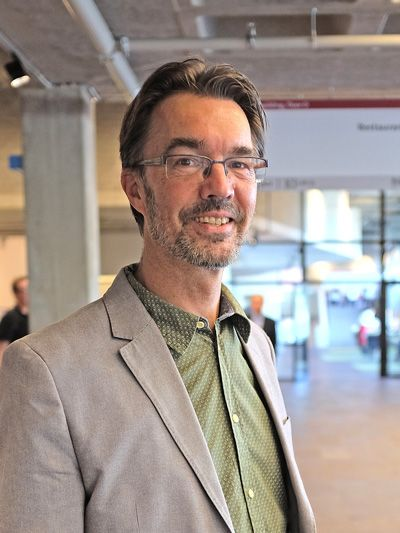
\includegraphics[width=0.5\linewidth]{deregt.jpg} \\
{\scriptsize Henk de Regt}

\vspace{1em}

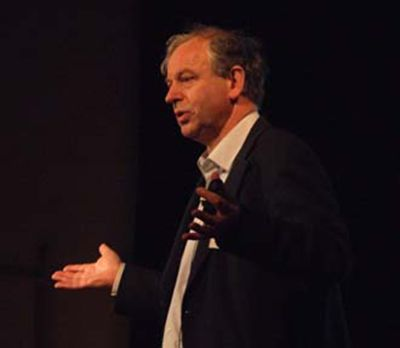
\includegraphics[width=0.5\linewidth]{dieks.jpg} \\
{\scriptsize Dennis Dieks}

\end{columns}

\end{frame}

\begin{frame}

  \begin{itemize}
  \item De Regt and Dieks offer us a ``theory'' of what scientific
    understanding is --- or, at least, what its characteristic signs
    are
  \item Their account of understanding is a successor to several
    competing accounts of scientific explanation that were offered
    between 1960 and 2000
  \item Their account is intended to show that understanding is
    \textbf{epistemically relevant}
  \end{itemize}

\end{frame}

\section{What drives science?}

\begin{frame}{What Drives Science?}

\begin{columns}
% Left column: text
\column{0.6\textwidth}
\small
\textbf{Empiricism:} The goal of science is to predict the results of experiments.

\vspace{0.5em}
\begin{quote}
  “According to empiricists such as Hempel and van Fraassen, the
  epistemic aim of science is (roughly stated) the production of
  factual knowledge about natural phenomena.” (p. 141)
\end{quote}

\vspace{0.5em}
\begin{itemize}
  \item 1870–1950: Ernst Mach, Logical Positivism
  \item 1960– : Carl Hempel, Bas van Fraassen, Brad Wray
\end{itemize}

% Right column: image
\column{0.4\textwidth}
\centering

\includegraphics[width=0.9\linewidth]{image.jpg} \\
\vspace{0.5em}
{\scriptsize Bas van Fraassen,\\ \textit{The Scientific Image} (1980)}

\end{columns}

\end{frame}


\begin{frame}{What drives science?}

  \begin{itemize}
  \item \textbf{Scientific Realism:} Science aims to \textbf{explain}
    phenomena.
    \begin{itemize}
    \item The realist reaction to logical positivism has been dominant
      among philosophers in the anglo-american tradition since the
      1960s
    \end{itemize}
  \end{itemize}

\end{frame}

\begin{frame}

  \begin{itemize}
  \item Empiricists see the aim of science as knowing \textbf{that}
    while realists see the aim of science as knowing \textbf{why}
  \item Is understanding needed?
  \end{itemize}

\end{frame}

\begin{frame}{What drives science?}

  \begin{itemize}
  \item De Regt and Dieks: ``We will argue that achieving
    understanding is among the general (macro-level) aims of science''
    (p 140)
  \item ``Understanding is an inextricable element of the aims of
    science'' (p 142)
  \end{itemize}

\end{frame}


\section{Philosophy of science background}

\begin{frame}{Origins of logical positivism}

  \begin{columns}
  \begin{column}{0.55\textwidth}
    Gottlob Frege (1848--1925) was a German mathematician who argued
    for a strict separation of the (objective) logical from the
    (subjective) psychological
    \begin{itemize}
    \item He was a key player in formalizing the logical foundations
      of mathematics
    \item The validity of a ``inference'' is an objective fact,
      independent of any person who is thinking about it
    \end{itemize}
  \end{column}

\begin{column}{0.45\textwidth}
  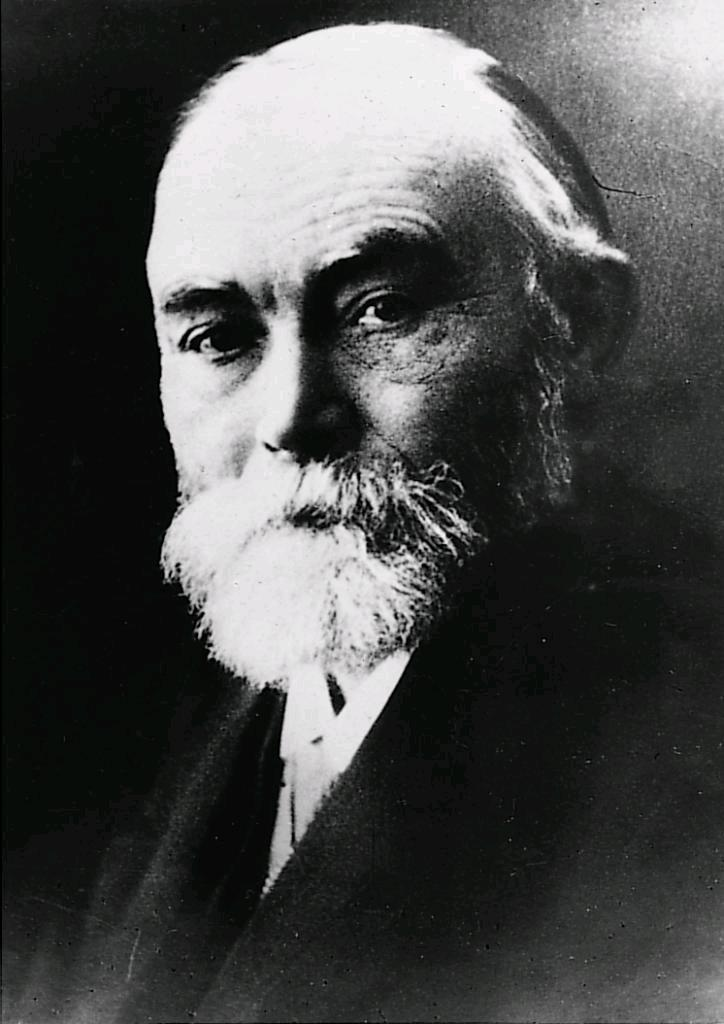
\includegraphics[scale=0.15]{frege}
\end{column}
\end{columns}  

\end{frame}

\begin{frame}{Origins of logical positivism}
 \begin{columns}
  \begin{column}{0.55\textwidth}
    \begin{itemize}
    \item Rudolf Carnap (1891--1970) was a student of Frege, also
      trained in physics and philosophy
    \item Carnap's idea: apply Fregean logical rigor to the empirical
      sciences --- \textbf{logic of science program}  
    \end{itemize}
    \end{column}
    \begin{column}{0.35\textwidth}
      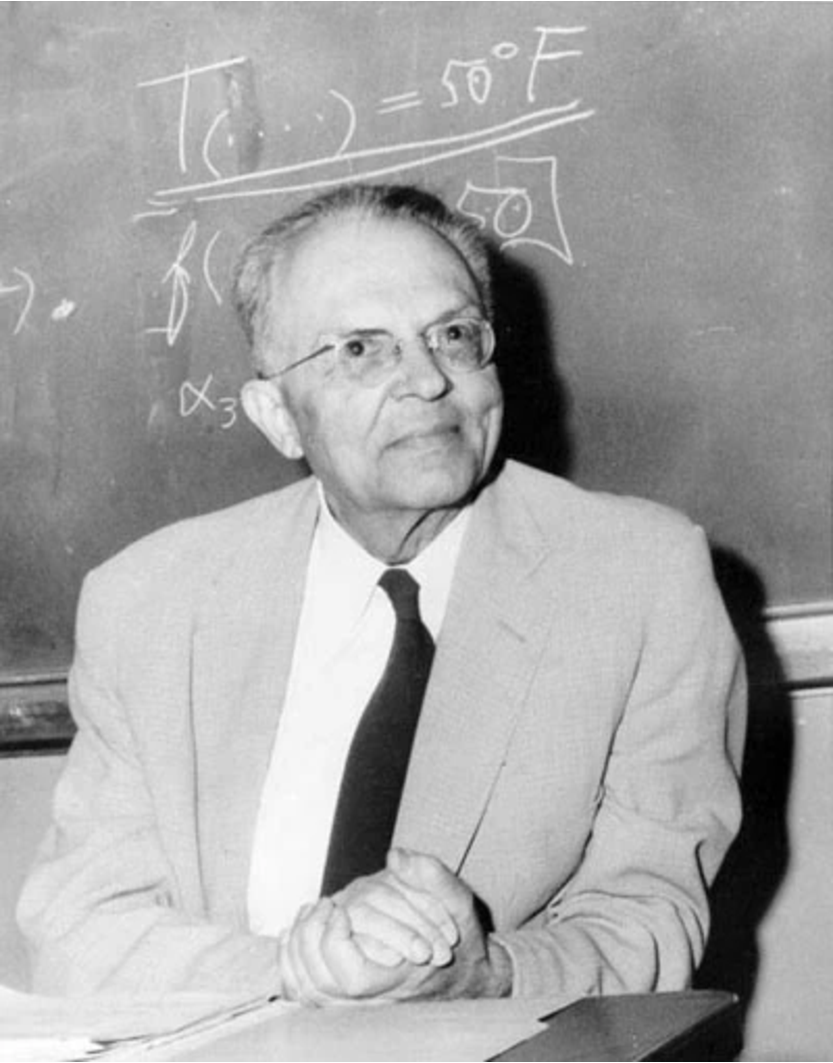
\includegraphics[scale=0.3]{carnap.pdf}
    \end{column}
   \end{columns}

\end{frame}

\begin{frame}{A scientific theory of science?}

  \begin{itemize}
  \item Carnap was concerned with talking \emph{about} science in a
    scientifically rigorous fashion
  \item Mathematical rigor: definable in some well-understood formal
    system
  \item At first, Carnap thought that not even ``truth'' qualified as
    a scientifically legitimate concept
  \item He never recognized ``explains'' as a scientifically
    legitimate concept
  \end{itemize}

\end{frame}

\begin{frame}{The post-war realist turn}

  ``To explain the phenomena in the world of our experience, to answer
  the question `why?' rather than only the question `what?', is one of
  the foremost objectives of all rational inquiry; and especially,
  scientific research in its various branches strives to go beyond a
  mere description of its subject matter by providing an explanation
  of the phenomena it investigates.'' (Hempel and Oppenheim 1948)

\end{frame}

\begin{frame}{Carl Hempel}

  \begin{columns}
    \begin{column}{0.6\textwidth}
  \begin{itemize}
  \item Carl Hempel (1905--1997) was a member of the Berlin Circle,
    and immigrated to the US in 1937
  \item Hempel: ``explains'' is a worldly relation that holds between
    facts, quite independent of the person (or group) of people
    considering them
  \item The goal of science is to find the (objective) explanation for
    the phenomena
  \end{itemize}
\end{column}

      \begin{column}{0.35\textwidth}
        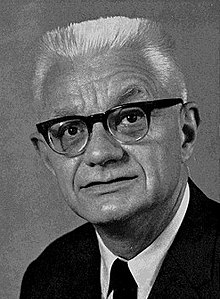
\includegraphics[scale=0.4]{hempel}
      \end{column}
\end{columns}
  
\end{frame}


\begin{frame}

  \begin{columns}
  \begin{column}{0.6\textwidth}
    ``Such expressions as `realm of understanding' and
    `comprehensible' do not belong to the vocabulary of logic, for
    they refer to the psychological and pragmatic aspects of
    explanation.'' (Carl Hempel)
  \end{column}

  \begin{column}{0.4\textwidth}
    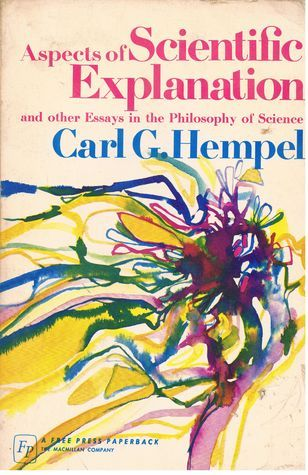
\includegraphics[scale=2.5]{aspects}
  \end{column}
  \end{columns}

\end{frame}

\begin{frame} 

  ``Carl Hempel \dots argued that `understanding' is subjective and
  merely a psychological by-product of scientific activity and is,
  therefore, not relevant for the philosophy of science.''  (Krenn et
  al., p 762)

\end{frame}

\section{Theories of scientific explanation}

\begin{frame}{Major Accounts of Scientific Explanation (Historical Overview)}

\scriptsize
\begin{itemize}
  \item \textbf{Hempel (1940s–60s)}: Deductive-Nomological Model
    \begin{itemize}
      \item Explanation = logical deduction from laws + initial conditions
      \item Criticized for overgenerating (irrelevance) and symmetry
    \end{itemize}

  \item \textbf{Salmon (1970s–80s)}: Causal Models
    \begin{itemize}
      \item Statistical relevance $\Rightarrow$ causal relevance
      \item Explanation = tracing causal/mechanical processes
    \end{itemize}

  \item \textbf{Friedman \& Kitcher (1970s–80s)}: Unificationist Accounts
    \begin{itemize}
      \item Explanation = increased understanding via unification
      \item Fewer independent assumptions; general argument patterns
    \end{itemize}
\end{itemize}

\end{frame}




\begin{frame}{Deductive nomological account}

  Nomos = law

  \medskip Hempel proposed a general schema according to which a fact
  $E$ (the explanandum) is explained by being deduced logically from a
  covering law $L$ and an initial condition $C$ (the explanans).

  \vfill \begin{tabular}{ll}
  Initial condition \\
  Law \\ \hline
  Explanandum (to be explained)
  \end{tabular}

\end{frame}

\begin{frame}{DN both over- and undergenerates}

  \begin{itemize}
  \item DN undergenerates: There are legitimate scientific
    explanations that do not match the strict, DN format
  \item Hempel nuanced the DN account to include statistical
    explanations
  \item DN overgenerates: There are pseudo-explanations that match the
    strict DN format
    \begin{itemize}
    \item Asymmetry: Flagpole
    \item Relevance: Birth control pills
    \end{itemize}
  \end{itemize}

\end{frame}

\begin{frame}{Flagpole and Shadow: A Problem for Hempel}

\begin{columns}
\column{0.55\textwidth}

\scriptsize
\vspace{-0.5em}
\textbf{D-N Explanation (Hempel):}
\begin{itemize}
  \item Given: flagpole height $h$, sun angle $\theta$
  \item Law: $\tan(\theta) = \frac{h}{s}$
  \item Deduce: shadow length $s$
\end{itemize}

\vspace{0.5em}
\textbf{But also:}
\begin{itemize}
  \item Given $s$ and $\theta$, deduce $h$
\end{itemize}

\vspace{0.5em}
\textbf{What's wrong?}
\begin{itemize}
  \item Both directions are deductive...
  \item ...but only one feels explanatory.
\end{itemize}

\column{0.45\textwidth}

\begin{tikzpicture}[scale=1.2, every node/.style={font=\scriptsize}]
  % Ground
  \draw[thick] (0,0) -- (3.5,0);

  % Flagpole
  \draw[very thick] (0,0) -- (0,3);
  \node[left] at (0,1.5) {$h$};

  % Shadow
  \draw[thick] (0,0) -- (3,0);
  \node[below] at (1.5,0) {$s$};

  % Sun rays and triangle
  \draw[dashed] (0,3) -- (3,0);
  \node at (2.6,1.6) {$\theta$};

  % Right angle box
  \draw (0,0) rectangle +(0.2,0.2);
\end{tikzpicture}

\end{columns}

\end{frame}


\begin{frame}{Hempel's D-N Model Overgenerates}

\vspace{-0.5em}
\textbf{Premises (Laws + Initial Conditions):}
\begin{itemize}
  \item[(L)] All males who take birth control pills regularly fail to get pregnant.
  \item[(C)] John Jones is a male who has been taking birth control pills regularly.
\end{itemize}

\vspace{0.5em}
\textbf{Conclusion (E):}
\begin{itemize}
  \item[(E)] John Jones fails to get pregnant.
\end{itemize}

\vspace{0.5em}
\textbf{Problem:}
\begin{itemize}
  \item The derivation is logically valid under the D-N model.
  \item But it fails to identify a genuine \textit{explanatory} relation.
  \item Taking birth control pills is irrelevant to John's failure to become pregnant.
\end{itemize}

\vspace{0.5em} \textbf{Conclusion:} D-N explanation captures logical
derivability, but not explanatory relevance.

\end{frame}



\begin{frame}

  \begin{columns}
    \begin{column}{0.6\textwidth}
      \begin{itemize}
      \item For more than forty years, philosophers debated about the
        ``right'' account of scientific explanation.
      \item ``Newton-Smith (2000) observes that fifty years of
        discussion have not led to consensus, but, on the contrary, to
        many rival models of explanation.''
      \end{itemize}
    \end{column}
    \begin{column}{0.4\textwidth}
      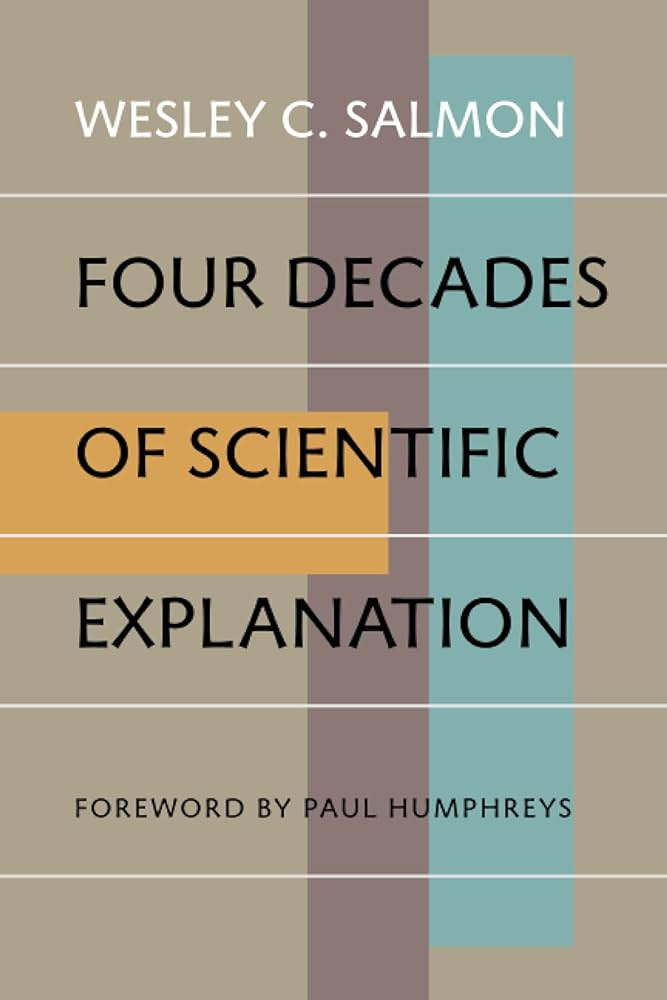
\includegraphics[scale=0.15]{decades}
    \end{column}
  \end{columns}


\end{frame}

\begin{frame}{Causal-mechanical account}

  \begin{itemize}
  \item A natural addendum to the DN account of explanation would be
    to require that the explanans is \textbf{causally relevant} to the
    explanandum.
  \item Wesley Salmon developed the idea that a scientific explanation
    is a description of the causal mechanism that results in the
    production of the phenomenon.  \end{itemize}

\end{frame}

\begin{frame}{Causal-mechanical account}

  \begin{itemize}
  \item The causal-mechanical account taps into the old tradition of
    mechanistic explanation (and visualizability)
  \end{itemize}



\end{frame}

\begin{frame}{Unificationist account}

  ``Science advances our understanding of nature by showing us how to
  derive descriptions of many phenomena, using the same patterns of
  derivation again and again, and, in demonstrating this, it teaches
  us how to reduce the number of types of facts we have to accept as
  ultimate (or brute).'' (Philip Kitcher)

\end{frame}

\begin{frame}{Stalemate}

  \begin{itemize}
  \item Proved beyond difficult to isolate the core idea of
    \textbf{explanation} that holds throughout all the different
    sciences
  \item The methodology of ``whatever examples I can remember from
    when I was a physics student'' was recognized as unacceptable
  \end{itemize}

\end{frame}

\section{Resurrecting ``understanding''}

\begin{frame}{Against the old critique of understanding}

  \begin{itemize}
  \item ``The present paper argues, \emph{pace} Newton-Smith, that
    understanding can play the desired unifying role.'' (p 137)
  \item ``Should we rely on the view of practicing scientists...?'' (p
    138)
  \end{itemize}

\end{frame}
\begin{frame}

  \begin{itemize}    
  \item De Regt and Dieks argue that understanding is an
    \textbf{epistemically relevant} concept.  \newline ``We will argue
    that understanding ... is epistemically relevant'' (p 138)
  \item De Regt and Dieks argue that understanding transcends
    individual psychology \newline ``We will argue that understanding
    ...  transcends the domain of individual psychology.'' (p. 138)
  \end{itemize}

\end{frame}

\begin{frame}{Understanding is contextual}

  \begin{itemize}
  \item HH: A phenomenon can be \ul{contextual} and yet be
    second-order objective
  \item For example, it is second-order objective that ``Oslo is less
    than 500km from us''
  \item HH: de Regt and Dieks have not yet shown the sense in which
    understanding or intelligibility is second-order objective
  \end{itemize}

\end{frame}

\nocite{*}

\begin{frame}[allowframebreaks]{Selected References}
\printbibliography[heading=none, keyword=scientific-explanation]
\end{frame}

\section{Mathematization}

\begin{frame}

  \begin{itemize}
  \item In this second part, we look at an earlier complaint that
    mathematization was ruining physics
  \item Accusation: Isaac Newton is reducing our physical
    understanding by making everything mathematical
  \end{itemize}

\end{frame}

\begin{frame}
\begin{itemize}
\item This case study has wide ranging implications
  \begin{itemize}
  \item Interdisciplinarity
    \begin{itemize}
    \item How can math and physics work together if their goals are
      different?
    \item Are contemporary universities hurting science by building
      ``disciplinary silos''?
    \end{itemize}
  \item Good and bad uses of mathematics
  \item Methodological pluralism
   \end{itemize}
\end{itemize}

\end{frame}


\section{From Aristotle to Newton}


\begin{frame}{Physics before Newton}

  \begin{enumerate}
  \item In the middle ages, there was a kind of qualitative
    proto-physics that built on the work of the Greek philosopher
    Aristotle (384--322 BCE)
  \item The mechanical philosophy (Cartesian physics)
  \end{enumerate}

\end{frame}

\begin{frame}{Aristotelian physics}

  \begin{itemize}
  \item Does \ul{not} use mathematics or equations
  \item Predictions are qualitative
    \begin{itemize}
    \item E.g. rocks tend to fall because they are made of ``earthy
      stuff'' \end{itemize}
  \item Physical objects are assumed to have a sort of built in code
    that determines their behavior --- their \kw{form}
  \end{itemize}

\end{frame}


\begin{frame}{The revolution of Galileo and Descartes}

  \begin{itemize}
  \item The \kw{mechanical philosophy} was a paradigm for physics that
    came between the Aristotelian and Newtonian periods
  \item Heralded by Galileo Galilei (1564--1642)
    \begin{itemize}
    \item Precise, quantitative description of motion
    \item Elimination of \kw{occult qualities}, e.g. Aristotelian
      forms
    \end{itemize}
  \end{itemize}

\end{frame}

\begin{frame}{The mechanical philosophy}

  \begin{itemize}
  \item Articulated by Ren{\'e} Descartes (1596--1650)
  \item Descartes wants to reduce everything to \kw{configuration}
    \begin{itemize}
    \item No force
    \item Mass is not a fundamental quantity, but a description of
      density of matter
    \item Velocity (momentum) is not a \kw{fundamental} quantity, but
      a summary of change of location over time
    \end{itemize}
  \end{itemize}

\end{frame}

\begin{frame}
  \begin{itemize}
  \item Descartes has algebraic geometry: equations and shapes
  \item Descartes does not have derivatives
  \item Descartes does not have vector quantities
  \item Despite the use of mathematics, the idea of explanation is
    \emph{mechanical}: contact, pushing, pulling 
  \end{itemize}
\end{frame}

\begin{frame}

  \begin{itemize}
  \item ``For the whole of the seventeeth century and most of the
    eighteenth, to `explain' a physical phenomenon meant to give the
    physical mechanism involved in its production.'' (Gingras, p 398)
  \item ``\dots science as a kind of verbal physics based on clear and
    distinct ideas.'' (Gingras, p 399)
  \end{itemize}

  %% TO DO: Picture of Principia 

  %% TO DO: Newton's objections to Cartesian physics (De Gravitatione)


\end{frame}

\begin{frame}{Cartesian vortices}

  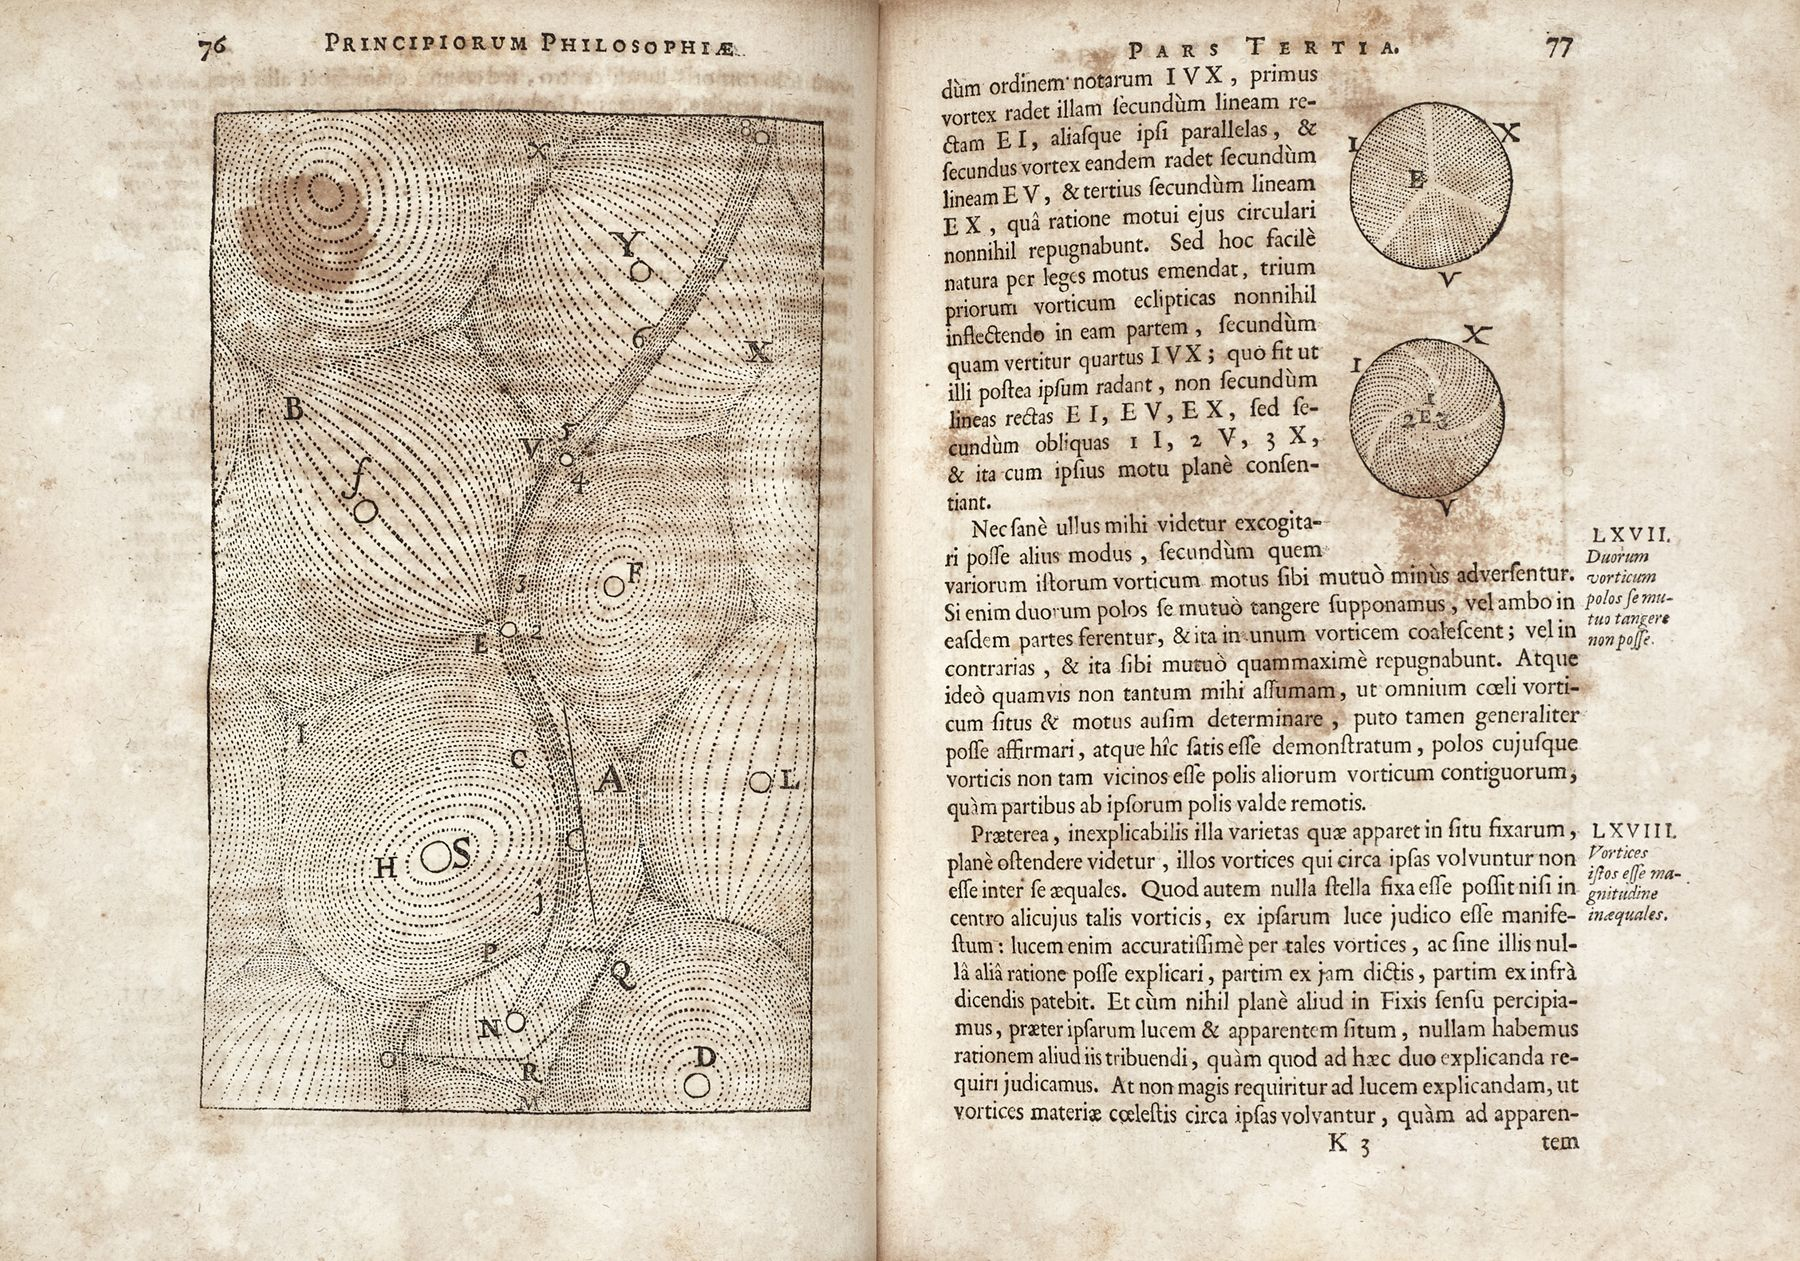
\includegraphics[scale=0.15]{vortices.jpeg}

\end{frame}
%% vortices


\begin{frame}{Mathematization of the concept of force} 

  ``Though Galileo preceded Newton in applying geometry to free fall,
  he did not concern himself with the \kw{efficient cause} of that
  fall and left that aspect outside his mathematics. The
  counter-intuitive effects of the mathematization of physical
  phenomena only began to be perceived with the development of
  dynamics, that is, that mathematization of the concept of force, as
  the cause of change in the state of motion.'' (Gingras, p 387)

  \[ F = m\ddot{q} \]


\end{frame}

\begin{frame}

  ``The publication of Newton's \emph{Principia} marks the beginning
  of this shift where mathematical explanations came to be preferred
  to \kw{mechanical explanations} \emph{when the latter did not
    conform to calculations}.'' (Gingras, p 398)

\end{frame}


\begin{frame}

  ``\dots only true mechanical contact between the parts of a plenum
  could be considered a \emph{physical} explanation, whereas Newton
  had simply posited mathematical forces, which pertains to a
  different order of things, namely geometry, and thus could not
  constitute a true \kw{explanation} of physical phenomena.''
  (Gingras, p 399)


\end{frame}

%% Garber

\begin{frame}

  \begin{itemize}
  \item Historians and philosophers intend slightly different things
    with the question ``what were the reasons for the mathematization
    of physics?''
    \begin{itemize}
    \item Historians: what were the (external) causes that led to
      mathematization?
    \item Philosophers: what are the \textbf{reasons} for
      mathematization?
    \end{itemize}
  \item The philosopher's question is particularly relevant if we are
    considering what we plan to do going forward
  \end{itemize}


\end{frame}

\begin{frame}

  \begin{itemize}
  \item In ``What did mathematics do to physics'', Gingras asks
    neither about the causes nor the reasons for mathematization, but
    about the effects it had

    ``It is thus the \emph{effects} rather than the causes (or
    reasons) of the mathematization of physics that I want to follow
    in this paper.'' (Gingras, p 384)
    
  \item Most interesting for us is the fierce resistance that Newton
    faced.

  \item Many physicists argued that Newton would destroy empirical
    science! 
  \end{itemize}

\end{frame}


\begin{frame}

  \begin{itemize}
  \item Gingras sorts the consequences of mathematization into three
    kinds
    \begin{enumerate}
    \item \kw{Social}: How mathematization affected people and their
      relations with each other
    \item \kw{Epistemological}: Gingras is using ``epistemological''
      not in the standard sense of ``what we know'', but in the
      peculiar sense of what kinds of \kw{explanations} were found
      acceptable
    \item \kw{Ontological:} How mathematization affected physicists'
      view of what exists
    \end{enumerate}

    
  \end{itemize}
\end{frame}

\section{Social consequences of mathematization}

\begin{frame}{Social consequences of mathematization}

  \begin{itemize}
  \item Summary: The mathematization of physics made understanding its
    results --- and judging them authoritatively --- only available to
    the mathematically adept
  \item Mathematization put a damper on a tradition of public
    engagement with physics
    \begin{itemize}
    \item Not ``public'' in the sense of the masses, but ``public'' in
      the sense of ``the wealthy and well educated, but not
      necessarily in the natural sciences''
    \end{itemize}
  \end{itemize}

\end{frame}

\begin{frame}

  \begin{itemize}
  \item ``Euler made plain that the price of entry into the club of
    legitimate practitioners was an adequate knowledge of
    mathematics.'' (Gingras, p 390)
  \item ``Once the boundaries were well defined and the gate keepers
    controlled access to the legitimate places of publication,
    outsiders could make their voices heard only in books or in
    magazines of general interest.'' (Gingras, p 391)
  \end{itemize}


\end{frame}

\begin{frame}

  \begin{itemize}
  \item ``It was this very `right to an opinion' without having the
    proper prior training that the mathematization of physics was
    putting into question.'' (Gingras, p 392)
  \item ``Paralleling the `rise of public science' \dots mathematics
    contributed to the rise of a `private science', accessible only to
    the adequately trained.'' (Gingras, p 393)
  \item ``Mathematization contributed to the formation of a relatively
    autonomous scientific field, with its control of access
    mechanisms.'' (Gingras, p 395)
  \end{itemize}
 
\end{frame}

\begin{frame}

  \begin{itemize}
  \item ``For d'Alembert, the era of verbal (or literary) physics was
    over; at least in matters concerning the Newtonian world system.''
    (Gingras, p 393)
  \item ``For them, less talented or less interested in investing long
    hours in abstruse mathematical calculations, the legitimacy of
    their verbal contributions to physics was threated by view like
    those put forward by d'Alembert.'' (Gingras, p 394)
  \end{itemize}

\end{frame}

\begin{frame}{What didn't the mechanical philosophers like about
    Newton's physics?}

  \begin{itemize}
  \item ``Privat de Moli{\'e}res thus clearly preferred the `\`a peu
    pr\`es' of vortex theory to the artificial geometrical precision
    of Newton's `metaphysical forces'. His critique of the excessive
    precision implicit in Newton's mathematization \dots '' (Gingras,
    p 389)
  \item ``This notion that nature does not suffer too much precision,
    was reminiscent of Aristotle'' (Gingras, p 389)
  \end{itemize}



\end{frame}

\begin{frame}

  \begin{itemize}
  \item ``Natural philosophy is and ought to be mathematics, that is,
    the science in which laws relating to quantity are treated
    according to the principles of accurate reasoning.'' (Maxwell
    1856)
  \end{itemize}


\end{frame}

\section{Epistemological consequences of mathematization}

\begin{frame}

  \begin{itemize}
  \item ``\dots it was the very meaning of the term `explanation' that
    was at stake in the discussions concerning the legitimacy of
    hypotheses.'' (Gingras, p 398)
  \item Recall that Newton said that he, unlike the Cartesians, didn't
    make hypotheses
  \item ``This episode shows that the evaluation criteria for what was
    to count as an acceptable `explanation' (of gravitation in this
    case) were shifting towards mathematics and away from mechanical
    explanations.'' (Gingras, p 398)
 \end{itemize}

\end{frame}

\begin{frame}

  \begin{itemize}
  \item ``Newton was in practice saying that mathematics was replacing
    verbal formulations as the final arbiter and true explanation of
    the phenomena.'' (Gingras, p 399)
  \item ``Newton had mixed physics with mathematics and thus explained
    physical phenomena mathematically.'' (Gingras, p 399)
  \end{itemize}
    
\end{frame}

\begin{frame}

  ``The implicit definition of the term `physics' used here by [Louis
  Bertrand] Castel is one related to the idea that physics provides
  mechanical explanations which should not be confused with
  mathematical explanations.'' (Gingras, p 400)
\end{frame}

\section{Ontological consequences of mathematization}

\begin{frame}

\begin{itemize}
\item \kw{Ontology} is the study of what exists
\item Physics surely has a special role in telling us what exists and
  how it behaves
  \begin{itemize}
  \item E.g. everything is subject to the law of gravity
  \end{itemize}
\item Some philosophers believe that physics is the final arbiter of
  ontology
  \begin{itemize}
  \item \kw{Reductionism} is the view that the things that appear in
    other sciences (molecules, genes, plants, animals, etc.) are
    ultimately just complex versions of the things that appear in
    physics
  \item \kw{Physicalism} is the view that every existing thing is made
    out of the things described in physics
  \end{itemize}
\end{itemize}

\end{frame}

\begin{frame}

  \begin{itemize}
  \item One reason some philosophers and physicists find QM
    unsatisfactory is because they don't think it has a clear ontology
  \item Is it a fundamental goal of physics to provide ontology?
  \end{itemize}

\end{frame}


\begin{frame}{Physics' standard dilemma about ontology}

  \begin{description}

  \item[Plenum views] There is ``stuff'' that fills space
    \begin{itemize}
    \item Aristotle
    \item Cartesian ``extended stuff''
    \item Wave theories
    \item Field theories (e.g. electromagnetism)
    \end{itemize}
  \item[Particle views] There are indivisible chunks of matter that
    are separated by empty space
    \begin{itemize}
    \item Lucretius' atoms
    \item Newton
    \end{itemize}
  \end{description}


\end{frame}

\begin{frame}

  \begin{itemize}
  \item ``In addition to making possible abstraction and
    generalization, the manipulation of symbols discussed by Biot and
    Maxwell were to have an important if often undesired and
    disturbing ontological effect.'' (Gingras, p 404)
  \end{itemize}
\end{frame}  


\begin{frame}{Does mathematization obviate ontology?}

  \begin{itemize}
  \item Gingras: Mathematization caused physicists to stop thinking
    about ontology in traditional terms
    \begin{itemize}
    \item ``Only a more detailed analysis could show that the
      \ul{desubstantialization of matter} was directly related to the
      mathematization process itself'' (p 406) \end{itemize}
  \item What does he mean by the ``desubstantialization of matter''?
  \end{itemize}  
\end{frame}

\begin{frame}

  \begin{itemize}
  \item ``Mathematics has had the tendency of redirecting the focus of
    inquiry towards the relational character of the elements, thus
    contributing to the transformation of concepts and practices.''
    (Gingras, p 406)
  \end{itemize}

\end{frame}



\begin{frame}{Structural realism}

\begin{itemize}
  \item What Gingras notices occuring in attitudes toward ontology is
    heralded by some physicists and philosophers as a positive
    movement in the direction of \kw{structuralism}
  \item Structural realism: physics is not interested in the natures
    of things, but only in their structural relations with each other
  \end{itemize}
   
\end{frame}


\section{Conclusion}

\begin{frame}{Mathematization in the 19th and 20th centuries}

  \begin{itemize}
  \item The mathematical overhead brought in by Newton was nothing in
    comparison to what happened in the 19th and 20th centuries
  \item Mathematics become more rigorous but also more abstract and
    distant from empirical reality
  \item The development of non-euclidean geometry undercut the idea
    that we are certain of the geometric structure of space
  \item The development of non-commutative matrix algebra was ---
    according to Bohr --- what allowed a rational formulation of
    quantum mechanics
 \end{itemize}


\end{frame}


\begin{frame}{For reflection going into week 6}

  \begin{itemize}
  \item Is what mathematics did to physics in the 17th and 18th
    centuries similar to what computers (machine learning, AI) are
    doing to physics now?
  \item Are we losing \kw{understanding}, or gaining a new kind?
  \item Should we fight the trend?
  \item How can we make best of the trend?
  \end{itemize}
\end{frame}


\begin{frame}{For reflection going into week 6} 

  \begin{itemize}
  \item What is the connection between mechanical explanation and the
    demand for visualizability (anskuelighed)?
  \item What is the connection between mechanical explanation and
    understanding?
  \end{itemize}
  
\end{frame}










\end{document}
%%% Local Variables:
%%% mode: latex
%%% TeX-master: t
%%% End:

  \begin{itemize}
  \item Algebraic geometry: Descartes
  \item Calculus: Newton
  \item Lagrangian and Hamiltonian mechanics 
  \item Tensors and differential equations: Maxwell
  \item Non-Euclidean geometry
    \begin{itemize}
      \item Undermined the idea that we may be certain of the
        Euclidean nature of the geometry of space
     \end{itemize}
  \item Riemannian geometry: Einstein 
  \item Wave equations
  \item Matrices: Jordan, Heisenberg
  \item Group theory and group representations: Wigner, Gell-Mann
  \end{itemize}


\end{frame}

\documentclass[fleqn]{beamer}

\usetheme[
  progressbar=frametitle,    % or try: 'none', 'foot'
  numbering=fraction,        % frame number / total
  sectionpage=none,
  subsectionpage=none
]{metropolis}


% Optional: custom keyword formatting
\newcommand{\kw}[1]{\textbf{#1}}


\section{A pluralist account of understanding}


\begin{frame}

  \begin{itemize}
  \item De Regt and Dieks: Understanding cannot be reduced to any of
    these particular accounts of scientific explanation
  \item HH: De Regt and Dieks do \emph{not} say that understanding
    requires at least one of these types of explanations. This seems
    like a defect of permissiveness in their account.
  \end{itemize}

\end{frame}  

\subsection{Causation not required for understanding}
  
\begin{frame}

\begin{itemize}
\item ``Salmon treats causality as a standard for intelligibility'' (p
  144)
\item ``Present-day scientific developments cast severe doubt on the
  alleged privileged status of [Salmon's] model of causal explanation
  as the way to scientific understanding.'' (p 145)
\item ``At the deepest levels of physical reality Salmon's concept of
  causality is highly problematic.'' (p 145)
\item ``Physics is full of examples that show that causal-mechanical
  explanation is not always the actually preferred manner of achieving
  understanding.'' (p 145)
\end{itemize}
  
\end{frame}


\begin{frame}{Quantum mechanics}

  \begin{itemize}
  \item ``Causal connections of this type \dots do not exist according
    to quantum theory in its standard interpretation.'' (p 145)
    \begin{itemize}
    \item Arguments against trajectories
    \item Bell non-locality
    \end{itemize}
  \end{itemize}
\end{frame}

\begin{frame}{Lorentz contraction}

  \begin{itemize}
  \item ``The usual way of making the contractions intelligible is by
    connecting them deductively to the basic posulates of special
    relativity (the relativity postulate and the light
    posulate). \dots Causal reasoning is not involved.''  (p 146)
  \item More controversial than De Regt and Dieks make it out to
    be. See Bell, ``How to teach special relativity'' or H. Brown,
    \emph{Physical Relativity} \end{itemize} 

\end{frame}

\begin{frame}{Deflection of light by matter in GTR}

  ``The just-mentioned example undermines the causal conception of
  understanding, because no causal chains were identified that are
  responsible for the deflection of the light.'' (p 157)

\end{frame}

\begin{frame}

  \begin{itemize}
  \item ``But even in pre-twentieth-century physics causal-mechanical
    explanation was not always the norm.'' (p 146)
  \item ``Between 1700 and 1850 action-at-a-distance rather than
    contact action and causal chains dominated the scientific scene.''
    (p 146)
  \end{itemize}

\end{frame}

\begin{frame}

  \begin{itemize}
  \item ``These facts are sufficient to cast doubt on the core idea
    that causality has a special status as \emph{the} fundamental,
    privileged standard of intelligibility.'' (p 146)
  \item ``It would be erroneous to maintain that visualization is
    essential for obtaining understanding.'' (p 156)
  \item ``The various intelligibility standards proposed by
    philosophers of science (e.g., visualizability, causality, and
    continuity) find a place in our approach as `tools' for achieving
    understanding: they can help to `see intuitively' the consequences
    of a scientific theory.'' (p 157)
  \end{itemize}

\end{frame}

\begin{frame}{Does causality have a privileged role?}

  \begin{itemize}
  \item ``By the guidance which analysis in terms of cause and effect
    has offered in many fields of human knowledge, the principle of
    causality has even come to stand as the ideal for scientific
    explanation.'' (Bohr 1948)
  \item ``The viewpoint of complementarity presents itself as a
    rational generalization of the very ideal of causality.'' (Bohr
    1948)
  \end{itemize}
  
\end{frame}


\subsection{Unification not required for understanding}

\begin{frame}

  \begin{itemize}
  \item ``Unification appears to be an effective tool for achieving
    understanding, but like causality it is one among a variety of
    tools.'' (p 149)
  \item ``The various intelligibility standards proposed by
    philosophers of science (e.g., visualizability, causality, and
    continuity) find a place in our approach as `tools' for achieiving
    understanding.'' (p 156--157)
  \end{itemize}

\end{frame}

\section{Understanding according to De Regt and Dieks}

\begin{frame}{Criterion for Understanding Phenomena}

  \textbf{CUP:} A phenomenon $P$ can be \textbf{understood} if a
  theory $T$ of $P$ exists that is intelligible.

\end{frame}

\begin{frame}{Criterion for the Intelligibility of Theories}
  
  \textbf{CIT:} A scientific theory $T$ is \textbf{intelligible} for
  scientists (in context $C$) if they can recognize qualitatively
  characteristic consequences of $T$ without performing exact
  calculations.


  \vspace{2em} ``What one wants in science is the ability to grasp how
  the predictions are brought about by the theory.'' (p 151)
  
\end{frame}

\begin{frame}[allowframebreaks]{Understanding Boyle’s Law via the Kinetic Theory}

\small
\textbf{Illustration of CUP and CIT:} How the kinetic theory provides understanding of gas behavior.

\vspace{0.5em}
\begin{itemize}
  \item \textbf{Qualitative model:} Boltzmann’s kinetic theory pictures a gas as a collection of freely moving molecules.
  \item \textbf{Temperature =} average kinetic energy of molecules.
  \item \textbf{Pressure =} cumulative force from molecular collisions with the container walls.
\end{itemize}

\vspace{1em}
\begin{center}
\begin{tikzpicture}[scale=0.8]
  % Container
  \draw[thick] (0,0) rectangle (5,3);

  % Molecules
  \foreach \x/\y in {1/1.5, 2/2.2, 3.5/1.7, 4/2.7, 1.5/0.8, 2.8/1, 4.5/1.2} {
    \filldraw[blue] (\x,\y) circle (0.08);
  }

  % Velocity arrows
  \draw[->,thick] (1,1.5) -- (1.4,1.8);
  \draw[->,thick] (2,2.2) -- (1.6,2.5);
  \draw[->,thick] (3.5,1.7) -- (3.1,1.4);
  \draw[->,thick] (4,2.7) -- (4.3,2.2);
  \draw[->,thick] (1.5,0.8) -- (1.7,1.2);
  \draw[->,thick] (2.8,1) -- (3.3,1.1);
  \draw[->,thick] (4.5,1.2) -- (4.1,0.9);

  % Label
  \node[align=center] at (2.5,-0.5) {\scriptsize Molecules move randomly and\\collide with container walls};

\end{tikzpicture}
\end{center}

\framebreak

\small
\textbf{Key insights (no equations):}
\begin{itemize}
  \item Adding heat $\Rightarrow$ molecules move faster $\Rightarrow$ more forceful, frequent collisions $\Rightarrow$ higher pressure.
  \item Reducing volume $\Rightarrow$ more collisions per unit area $\Rightarrow$ higher pressure (at constant temperature).
\end{itemize}

\vspace{0.5em}
\textbf{Conclusion:} The kinetic theory provides an intelligible, causal-mechanical picture that explains Boyle’s law qualitatively — in line with CUP and CIT.

\end{frame}



\begin{frame}{Problems with CIT?}

  \begin{itemize}
  \item CIT is ambiguous. Imagine a mechanical arm that pulls slips of
    paper out of a barrel, and always pulls out correct
    predictions. Would we be satisfied knowing how the mechanical arm
    operates?
  \item It seems that we would want to know how the mechanical arm
    manages to get the predictions right. We would want an explanation
    not of how it generates predictions, but of why it generates the
    right predictions 
    \end{itemize}



\end{frame}


\begin{frame}{Open questions}


  \begin{itemize}
  \item Does the account of De Regt and Dieks have any normative
    content? Or does it just point out the fairly obvious fact that
    scientific sub-communities have ideals for understanding?
  \item They point out that the Copenhagen-G{\"o}ttingen physicists
    found matrix mechanics to be intelligible, while most other
    physicists disagreed. (p 141)
  \end{itemize}



\end{frame}




\section{Mathematization}

\begin{frame}

  \begin{itemize}
  \item In the first part we talked about the foundational disputes
    about quantum mechanics
    \begin{itemize}
    \item The measurement problem purports to show that QM is
      inconsistent
    \item Even if QM is consistent, many people think it's
      unsatisfactory as a physical theory --- e.g. it doesn't provide
      understanding
    \end{itemize}
  \item Are we seeing ongoing resistance to paradigm change here?
    \begin{itemize}
    \item If so, what is the quantum paradigm?
    \end{itemize}
  \end{itemize}

\end{frame}


\begin{frame}

  \begin{itemize}
  \item In this second part, we look at an earlier complaint that
    mathematization was ruining physics
  \item Accusation: Isaac Newton is reducing our physical
    understanding by making everything mathematical
  \end{itemize}

\end{frame}

\begin{frame}
\begin{itemize}
\item This case study has wide ranging implications
  \begin{itemize}
  \item Interdisciplinarity
    \begin{itemize}
    \item How can math and physics work together if their goals are
      different?
    \item Are contemporary universities hurting science by building
      ``disciplinary silos''?
    \end{itemize}
  \item Good and bad uses of mathematics
  \item Methodological pluralism
   \end{itemize}
\end{itemize}

\end{frame}


\section{From Aristotle to Newton}


\begin{frame}{Physics before Newton}

  \begin{enumerate}
  \item In the middle ages, there was a kind of qualitative
    proto-physics that built on the work of the Greek philosopher
    Aristotle (384--322 BCE)
  \item The mechanical philosophy (Cartesian physics)
  \end{enumerate}

\end{frame}

\begin{frame}{Aristotelian physics}

  \begin{itemize}
  \item Does \ul{not} use mathematics or equations
  \item Predictions are qualitative
    \begin{itemize}
    \item E.g. rocks tend to fall because they are made of ``earthy
      stuff'' \end{itemize}
  \item Physical objects are assumed to have a sort of built in code
    that determines their behavior --- their \kw{form}
  \end{itemize}

\end{frame}


\begin{frame}{The revolution of Galileo and Descartes}

  \begin{itemize}
  \item The \kw{mechanical philosophy} was a paradigm for physics that
    came between the Aristotelian and Newtonian periods
  \item Heralded by Galileo Galilei (1564--1642)
    \begin{itemize}
    \item Precise, quantitative description of motion
    \item Elimination of \kw{occult qualities}, e.g. Aristotelian
      forms
    \end{itemize}
  \end{itemize}

\end{frame}

\begin{frame}{The mechanical philosophy}

  \begin{itemize}
  \item Articulated by Ren{\'e} Descartes (1596--1650)
  \item Descartes wants to reduce everything to \kw{configuration}
    \begin{itemize}
    \item No force
    \item Mass is not a fundamental quantity, but a description of
      density of matter
    \item Velocity (momentum) is not a \kw{fundamental} quantity, but
      a summary of change of location over time
    \end{itemize}
  \end{itemize}

\end{frame}

\begin{frame}
  \begin{itemize}
  \item Descartes has algebraic geometry: equations and shapes
  \item Descartes does not have derivatives
  \item Descartes does not have vector quantities
  \item Despite the use of mathematics, the idea of explanation is
    \emph{mechanical}: contact, pushing, pulling 
  \end{itemize}
\end{frame}

\begin{frame}

  \begin{itemize}
  \item ``For the whole of the seventeeth century and most of the
    eighteenth, to `explain' a physical phenomenon meant to give the
    physical mechanism involved in its production.'' (Gingras, p 398)
  \item ``\dots science as a kind of verbal physics based on clear and
    distinct ideas.'' (Gingras, p 399)
  \end{itemize}

  %% TO DO: Picture of Principia 

  %% TO DO: Newton's objections to Cartesian physics (De Gravitatione)


\end{frame}

\begin{frame}{Cartesian vortices}

  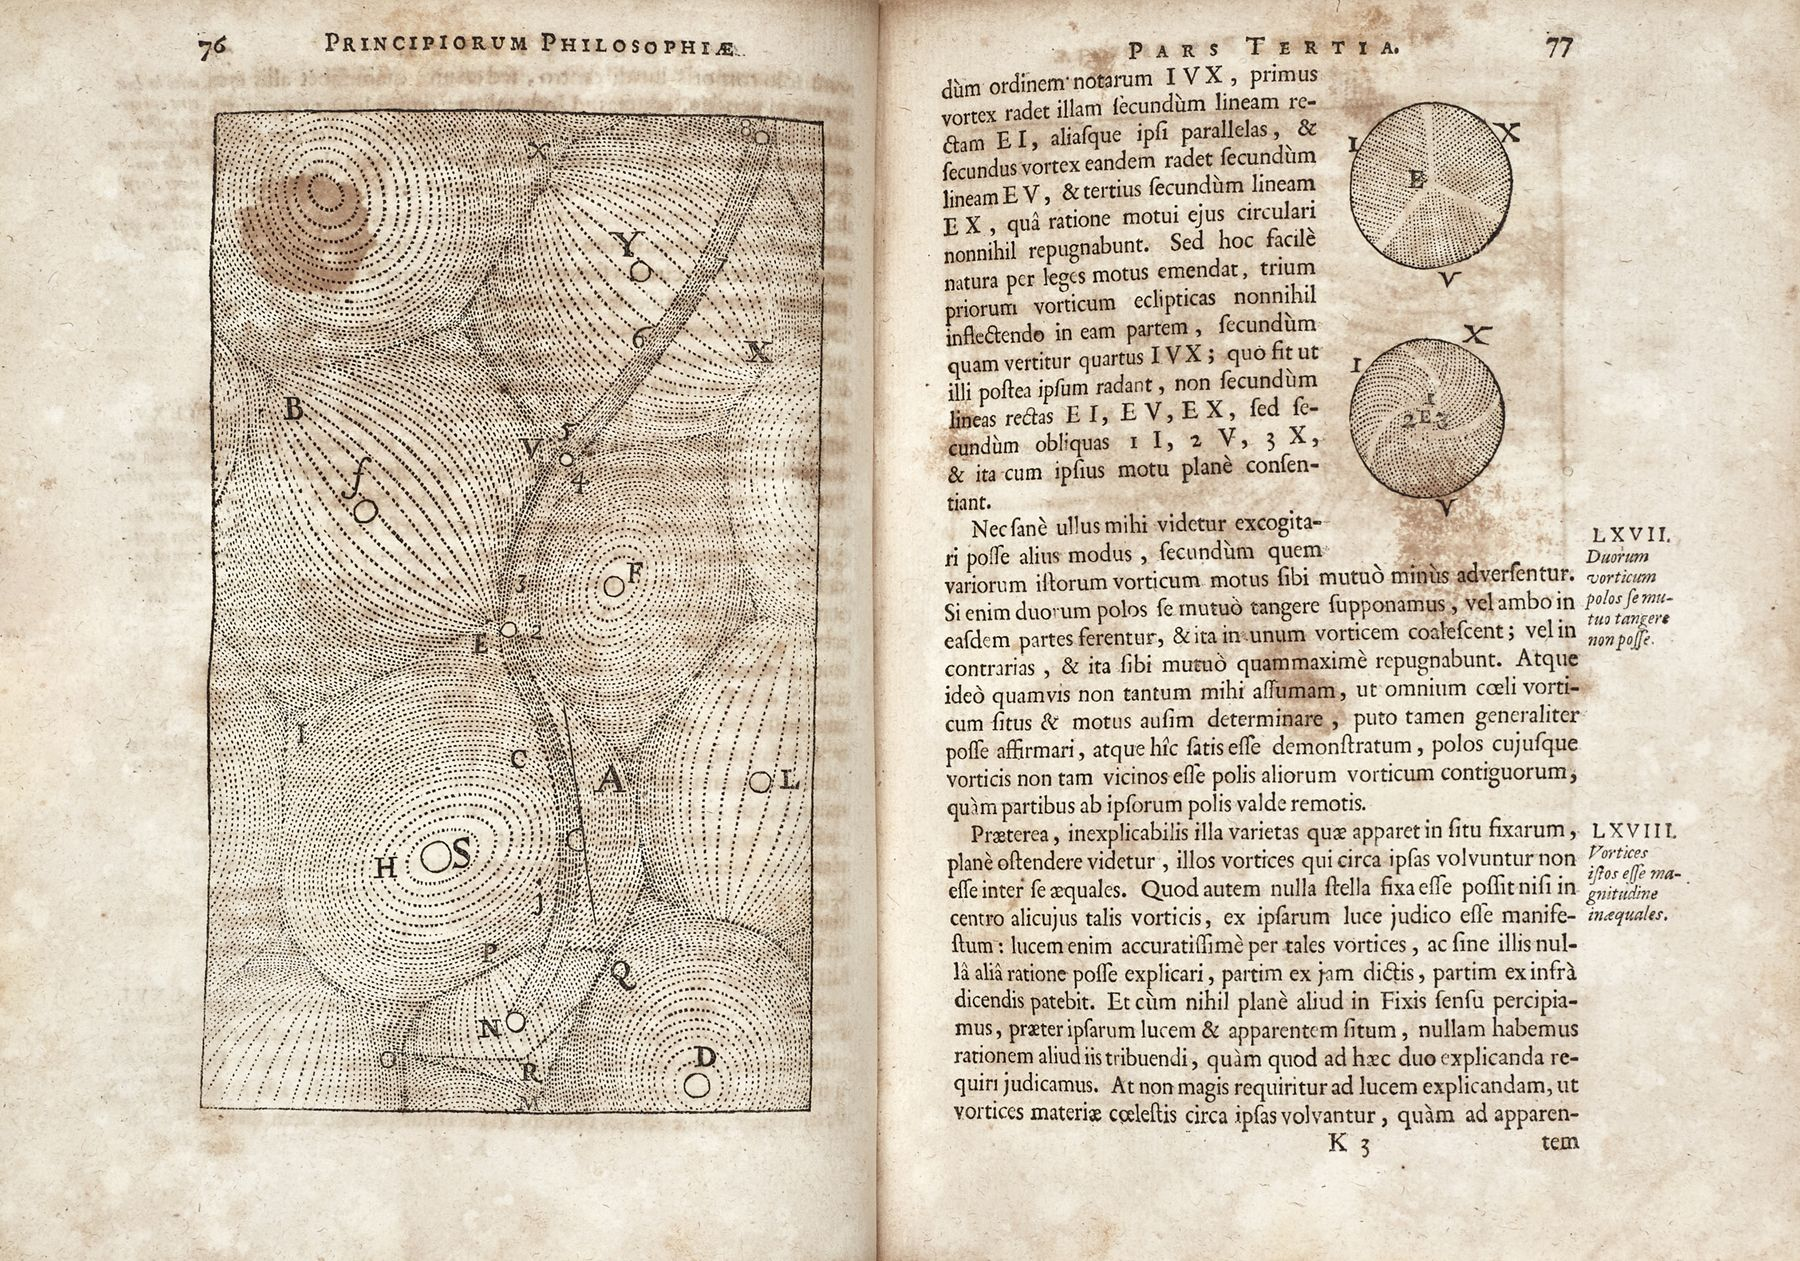
\includegraphics[scale=0.15]{vortices.jpeg}

\end{frame}
%% vortices


\begin{frame}{Mathematization of the concept of force} 

  ``Though Galileo preceded Newton in applying geometry to free fall,
  he did not concern himself with the \kw{efficient cause} of that
  fall and left that aspect outside his mathematics. The
  counter-intuitive effects of the mathematization of physical
  phenomena only began to be perceived with the development of
  dynamics, that is, that mathematization of the concept of force, as
  the cause of change in the state of motion.'' (Gingras, p 387)

  \[ F = m\ddot{q} \]


\end{frame}

\begin{frame}

  ``The publication of Newton's \emph{Principia} marks the beginning
  of this shift where mathematical explanations came to be preferred
  to \kw{mechanical explanations} \emph{when the latter did not
    conform to calculations}.'' (Gingras, p 398)

\end{frame}


\begin{frame}

  ``\dots only true mechanical contact between the parts of a plenum
  could be considered a \emph{physical} explanation, whereas Newton
  had simply posited mathematical forces, which pertains to a
  different order of things, namely geometry, and thus could not
  constitute a true \kw{explanation} of physical phenomena.''
  (Gingras, p 399)


\end{frame}

%% Garber

\begin{frame}

  \begin{itemize}
  \item Historians and philosophers intend slightly different things
    with the question ``what were the reasons for the mathematization
    of physics?''
    \begin{itemize}
    \item Historians: what were the (external) causes that led to
      mathematization?
    \item Philosophers: what are the \textbf{reasons} for
      mathematization?
    \end{itemize}
  \item The philosopher's question is particularly relevant if we are
    considering what we plan to do going forward
  \end{itemize}


\end{frame}

\begin{frame}

  \begin{itemize}
  \item In ``What did mathematics do to physics'', Gingras asks
    neither about the causes nor the reasons for mathematization, but
    about the effects it had

    ``It is thus the \emph{effects} rather than the causes (or
    reasons) of the mathematization of physics that I want to follow
    in this paper.'' (Gingras, p 384)
    
  \item Most interesting for us is the fierce resistance that Newton
    faced.

  \item Many physicists argued that Newton would destroy empirical
    science! 
  \end{itemize}

\end{frame}


\begin{frame}

  \begin{itemize}
  \item Gingras sorts the consequences of mathematization into three
    kinds
    \begin{enumerate}
    \item \kw{Social}: How mathematization affected people and their
      relations with each other
    \item \kw{Epistemological}: Gingras is using ``epistemological''
      not in the standard sense of ``what we know'', but in the
      peculiar sense of what kinds of \kw{explanations} were found
      acceptable
    \item \kw{Ontological:} How mathematization affected physicists'
      view of what exists
    \end{enumerate}

    
  \end{itemize}
\end{frame}

\section{Social consequences of mathematization}

\begin{frame}{Social consequences of mathematization}

  \begin{itemize}
  \item Summary: The mathematization of physics made understanding its
    results --- and judging them authoritatively --- only available to
    the mathematically adept
  \item Mathematization put a damper on a tradition of public
    engagement with physics
    \begin{itemize}
    \item Not ``public'' in the sense of the masses, but ``public'' in
      the sense of ``the wealthy and well educated, but not
      necessarily in the natural sciences''
    \end{itemize}
  \end{itemize}

\end{frame}

\begin{frame}

  \begin{itemize}
  \item ``Euler made plain that the price of entry into the club of
    legitimate practitioners was an adequate knowledge of
    mathematics.'' (Gingras, p 390)
  \item ``Once the boundaries were well defined and the gate keepers
    controlled access to the legitimate places of publication,
    outsiders could make their voices heard only in books or in
    magazines of general interest.'' (Gingras, p 391)
  \end{itemize}


\end{frame}

\begin{frame}

  \begin{itemize}
  \item ``It was this very `right to an opinion' without having the
    proper prior training that the mathematization of physics was
    putting into question.'' (Gingras, p 392)
  \item ``Paralleling the `rise of public science' \dots mathematics
    contributed to the rise of a `private science', accessible only to
    the adequately trained.'' (Gingras, p 393)
  \item ``Mathematization contributed to the formation of a relatively
    autonomous scientific field, with its control of access
    mechanisms.'' (Gingras, p 395)
  \end{itemize}
 
\end{frame}

\begin{frame}

  \begin{itemize}
  \item ``For d'Alembert, the era of verbal (or literary) physics was
    over; at least in matters concerning the Newtonian world system.''
    (Gingras, p 393)
  \item ``For them, less talented or less interested in investing long
    hours in abstruse mathematical calculations, the legitimacy of
    their verbal contributions to physics was threated by view like
    those put forward by d'Alembert.'' (Gingras, p 394)
  \end{itemize}

\end{frame}

\begin{frame}{What didn't the mechanical philosophers like about
    Newton's physics?}

  \begin{itemize}
  \item ``Privat de Moli{\'e}res thus clearly preferred the `\`a peu
    pr\`es' of vortex theory to the artificial geometrical precision
    of Newton's `metaphysical forces'. His critique of the excessive
    precision implicit in Newton's mathematization \dots '' (Gingras,
    p 389)
  \item ``This notion that nature does not suffer too much precision,
    was reminiscent of Aristotle'' (Gingras, p 389)
  \end{itemize}



\end{frame}

\begin{frame}

  \begin{itemize}
  \item ``Natural philosophy is and ought to be mathematics, that is,
    the science in which laws relating to quantity are treated
    according to the principles of accurate reasoning.'' (Maxwell
    1856)
  \end{itemize}


\end{frame}

\section{Epistemological consequences of mathematization}

\begin{frame}

  \begin{itemize}
  \item ``\dots it was the very meaning of the term `explanation' that
    was at stake in the discussions concerning the legitimacy of
    hypotheses.'' (Gingras, p 398)
  \item Recall that Newton said that he, unlike the Cartesians, didn't
    make hypotheses
  \item ``This episode shows that the evaluation criteria for what was
    to count as an acceptable `explanation' (of gravitation in this
    case) were shifting towards mathematics and away from mechanical
    explanations.'' (Gingras, p 398)
 \end{itemize}

\end{frame}

\begin{frame}

  \begin{itemize}
  \item ``Newton was in practice saying that mathematics was replacing
    verbal formulations as the final arbiter and true explanation of
    the phenomena.'' (Gingras, p 399)
  \item ``Newton had mixed physics with mathematics and thus explained
    physical phenomena mathematically.'' (Gingras, p 399)
  \end{itemize}
    
\end{frame}

\begin{frame}

  ``The implicit definition of the term `physics' used here by [Louis
  Bertrand] Castel is one related to the idea that physics provides
  mechanical explanations which should not be confused with
  mathematical explanations.'' (Gingras, p 400)
\end{frame}

\section{Ontological consequences of mathematization}

\begin{frame}

\begin{itemize}
\item \kw{Ontology} is the study of what exists
\item Physics surely has a special role in telling us what exists and
  how it behaves
  \begin{itemize}
  \item E.g. everything is subject to the law of gravity
  \end{itemize}
\item Some philosophers believe that physics is the final arbiter of
  ontology
  \begin{itemize}
  \item \kw{Reductionism} is the view that the things that appear in
    other sciences (molecules, genes, plants, animals, etc.) are
    ultimately just complex versions of the things that appear in
    physics
  \item \kw{Physicalism} is the view that every existing thing is made
    out of the things described in physics
  \end{itemize}
\end{itemize}

\end{frame}

\begin{frame}

  \begin{itemize}
  \item One reason some philosophers and physicists find QM
    unsatisfactory is because they don't think it has a clear ontology
  \item Is it a fundamental goal of physics to provide ontology?
  \end{itemize}

\end{frame}


\begin{frame}{Physics' standard dilemma about ontology}

  \begin{description}

  \item[Plenum views] There is ``stuff'' that fills space
    \begin{itemize}
    \item Aristotle
    \item Cartesian ``extended stuff''
    \item Wave theories
    \item Field theories (e.g. electromagnetism)
    \end{itemize}
  \item[Particle views] There are indivisible chunks of matter that
    are separated by empty space
    \begin{itemize}
    \item Lucretius' atoms
    \item Newton
    \end{itemize}
  \end{description}


\end{frame}

\begin{frame}

  \begin{itemize}
  \item ``In addition to making possible abstraction and
    generalization, the manipulation of symbols discussed by Biot and
    Maxwell were to have an important if often undesired and
    disturbing ontological effect.'' (Gingras, p 404)
  \end{itemize}
\end{frame}  


\begin{frame}{Does mathematization obviate ontology?}

  \begin{itemize}
  \item Gingras: Mathematization caused physicists to stop thinking
    about ontology in traditional terms
    \begin{itemize}
    \item ``Only a more detailed analysis could show that the
      \ul{desubstantialization of matter} was directly related to the
      mathematization process itself'' (p 406) \end{itemize}
  \item What does he mean by the ``desubstantialization of matter''?
  \end{itemize}  
\end{frame}

\begin{frame}

  \begin{itemize}
  \item ``Mathematics has had the tendency of redirecting the focus of
    inquiry towards the relational character of the elements, thus
    contributing to the transformation of concepts and practices.''
    (Gingras, p 406)
  \end{itemize}

\end{frame}



\begin{frame}{Structural realism}

\begin{itemize}
  \item What Gingras notices occuring in attitudes toward ontology is
    heralded by some physicists and philosophers as a positive
    movement in the direction of \kw{structuralism}
  \item Structural realism: physics is not interested in the natures
    of things, but only in their structural relations with each other
  \end{itemize}
   
\end{frame}


\section{Conclusion}

\begin{frame}{Mathematization in the 19th and 20th centuries}

  \begin{itemize}
  \item The mathematical overhead brought in by Newton was nothing in
    comparison to what happened in the 19th and 20th centuries
  \item Mathematics become more rigorous but also more abstract and
    distant from empirical reality
  \item The development of non-euclidean geometry undercut the idea
    that we are certain of the geometric structure of space
  \item The development of non-commutative matrix algebra was ---
    according to Bohr --- what allowed a rational formulation of
    quantum mechanics
 \end{itemize}


\end{frame}


\begin{frame}{For reflection going into week 6}

  \begin{itemize}
  \item Is what mathematics did to physics in the 17th and 18th
    centuries similar to what computers (machine learning, AI) are
    doing to physics now?
  \item Are we losing \kw{understanding}, or gaining a new kind?
  \item Should we fight the trend?
  \item How can we make best of the trend?
  \end{itemize}
\end{frame}


\begin{frame}{For reflection going into week 6} 

  \begin{itemize}
  \item What is the connection between mechanical explanation and the
    demand for visualizability (anskuelighed)?
  \item What is the connection between mechanical explanation and
    understanding?
  \end{itemize}
  
\end{frame}











\begin{frame}{A brief history of mathematization}

  \begin{itemize}
  \item Algebraic geometry: Descartes
  \item Calculus: Newton
  \item Lagrangian and Hamiltonian mechanics 
  \item Tensors and differential equations: Maxwell
  \item Non-Euclidean geometry
    \begin{itemize}
      \item Undermined the idea that we may be certain of the
        Euclidean nature of the geometry of space
     \end{itemize}
  \item Riemannian geometry: Einstein 
  \item Wave equations
  \item Matrices: Jordan, Heisenberg
  \item Group theory and group representations: Wigner, Gell-Mann
  \end{itemize}


\end{frame}










\end{document}
%%% Local Variables:
%%% mode: latex
%%% TeX-master: t
%%% End:



